%-----------------------------------------------------------------------------80
% SECTION TITLE
%-----------------------------------------------------------------------------80

\section{Subrutinas}  

%-----------------------------------------------------------------------------80
% CONTENT
%-----------------------------------------------------------------------------80


\begin{frame}[fragile]{Subrutinas}
 \begin{itemize}[<+(0)->]
  \item Una subrutina es un programa de menor orden jerárquico al principal.
  \item Tiene como objetivo llevar a cabo instrucciones ejecutables, por un subprograma de nivel superior, a través de una instrucción que llame a la subrutina.
  \item La sintaxis es la siguiente:\\
    \vspace{0.08cm} 
        \begin{minted}[linenos,autogobble]{fortran}
        subroutine <nombre><argumentos (ficticios)>
        !instrucciones de declaración de los argumentos (ficticios)
        !instrucciones de declaración de los objetos locales
        !instrucciones ejecutables
        end subroutine <nombre>
        \end{minted}
    donde los <argumentos (ficticios)>, en caso de uso, son los objetos sobre los cuales la subrutina trabajará preferentemente.
  \item La subrutina es llamada por un subprograma por medio de la intrucción CALL
    \vspace{0.08cm} 
        \begin{minted}[linenos,autogobble]{fortran}
        <identificacion unidad programatica>
        :
        call <nombre><argumentos (usasdos)>
        :
        end subroutine <unidad programática>
        \end{minted}  
 \end{itemize}
\end{frame}


\begin{frame}[fragile]{Subrutinas}
  \vspace{1cm}
  \begin{figure}
    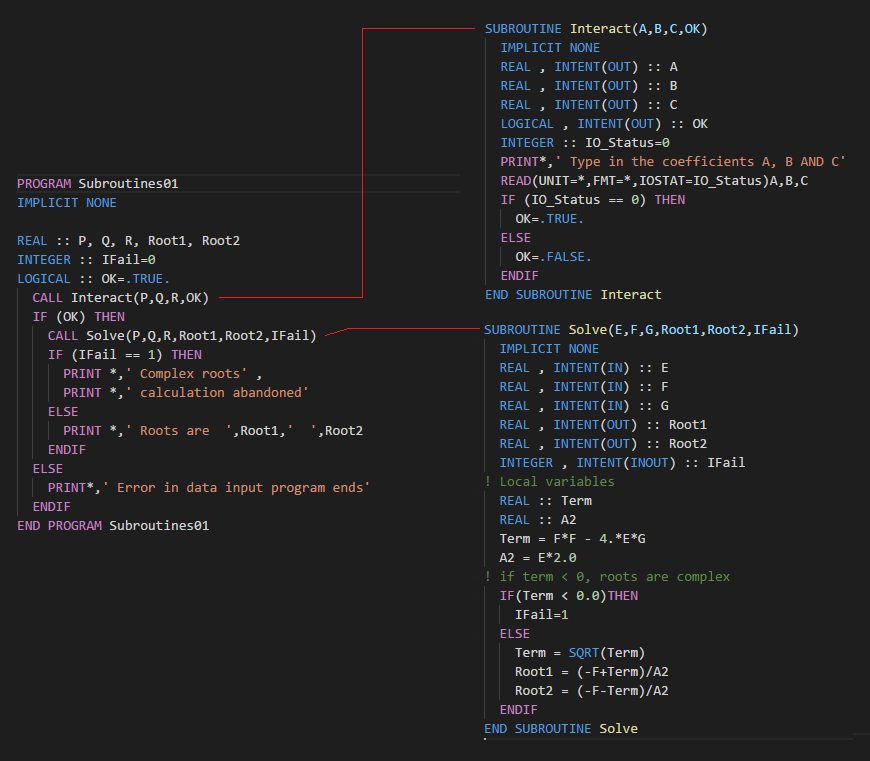
\includegraphics[width=0.7\textwidth]{./resources/subroutines.png}
    \caption*{Uso de subrutinas en Fortran}
  \end{figure}
\end{frame}


\subsection{Argumentos ficticios}


\begin{frame}[fragile]{Declaración de Argumentos ficticios}
 \begin{itemize}[<+(0)->]
  \item Los argumentos ficticios pueden ser variables, funciones, subrutinas, arreglos, punteros o procedimentos de módulo.
  \item Existe un bloque de instrucciones que permite declarar argumentos ficticios de una subrutina:
  \item [-] \emph{intent}(in): variables y arreglos cuyos valores permiten recibir información proporcionada por el subprograma que llama a la subrutina. Los valores no pueden ser modificados por la subrutina (comportamiento local).
  \item [-] \emph{intent}(on): variables y arreglos cuyos valores permiten devolver información, además de albergar resultados de un subprograma. Estos pueden ser modificados por la subrutina.
  \item [-] \emph{intent}(inout): variables y arreglos cuyos valores a la entrada pueden ser modificados (argumentos mixtos).
 \end{itemize}
\end{frame}

\begin{frame}[fragile]{Declaración de Argumentos ficticios}
\textbf{Declaración de arreglos}
 \begin{itemize}[<+(1)->]
  \item Primera regla: el tamaño de los arreglos empleados debe ser mayor o igual que el de los ficticios.  
   \vspace{0.15cm}
      \begin{minted}[linenos,autogobble]{fortran}
      REAL , ALLOCATABLE , DIMENSION &
      (:,:)::One,Two,Three,One_T
      INTEGER :: I,N
      INTERFACE
        SUBROUTINE Matrix_bits(A,B,C,A_T,N)
        IMPLICIT NONE
        INTEGER, INTENT(IN):: N
            REAL, DIMENSION (:,:), INTENT(IN) :: A,B
            REAL, DIMENSION (:,:), INTENT(OUT) :: C,A_T
        END SUBROUTINE Matrix_bits
      END INTERFACE
       PRINT *,'Input size of matrices'
       :
      \end{minted} 
 \end{itemize}
\end{frame}

\begin{frame}[fragile]{Declaración de Argumentos ficticios}
 \begin{itemize}[<+(0)->]
 \item Segunda regla: establecer correctamente la relación entre los elementos de ambos arreglos.
  \vspace{0.15cm}
      \begin{minted}[linenos,autogobble]{fortran}
      SUBROUTINE Matrix_bits(A,B,C,A_T,N) !Véase subroutines06.f95
       IMPLICIT NONE
       INTEGER, INTENT(IN):: N
       REAL, DIMENSION (:,:), INTENT(IN) :: A,B
       REAL, DIMENSION (:,:), INTENT(OUT) :: C,A_T
       INTEGER:: I,J, K
       REAL:: Temp
            !begining of matrix multiplication C = AB  
       DO I=1,N                         
           DO J=1,N
              Temp=0.0
              DO K=1,N
                 Temp = Temp + A(I,K) * B (K,J)
              END DO
                 C(I,J) = Temp
           END DO
        END DO
       :    !Calculate A_T transpose of A      !set A_T to be transpose matrix A
      END SUBROUTINE Matrix_bits
      \end{minted} 
 \end{itemize}
\end{frame} 

\begin{frame}[fragile]{Declaración de Argumentos ficticios}
\textbf{Declaración de cadenas de caracteres}
 \begin{itemize}[<+(1)->]
  \item La forma más conveniente es fijando la longitud de la cadena.
      \begin{minted}[linenos,autogobble]{fortran}
      SUBROUTINE subrutina(ciudad)
        CHARACTER(len=10)::ciudad
        :
      END SUBROUTINE subrutina
      \end{minted}
    \vspace{0.1cm}    
  \item De manera explícita, por medio de un argumento tipo INTEGER.
      \begin{minted}[linenos,autogobble]{fortran}
      SUBROUTINE subrutina(n, ciudad)
        INTEGER, INTENT(IN)::n
          CHARACTER(len=n), INTENT(INOUT)::ciudad
          :
      END SUBROUTINE subrutina
      \end{minted}
    \vspace{0.1cm} 
  \item De manera implícita, utilizando el símbolo "*"
      \begin{minted}[linenos,autogobble]{fortran}
      SUBROUTINE subrutina(ciudad)
        CHARACATER(len=*) INTENT(INOUT)::ciudad
        :
          n=len(ciudad) !da la longitud de la cadena del argumento en uso.
        :
      END SUBROUTINE subrutina
      \end{minted} 
 \end{itemize}
\end{frame}


\subsection{Objetos locales}

\begin{frame}[fragile]{Declaración de Objetos locales}
 \begin{itemize}[<+(0)->]
  \item Los objetos locales son de uso exclusivo de una subrutina y no utilizados por subprogramas de nivel superior.
  \item Para conservar los valores de las variables y arreglos locales de una llamada a otra, es necesario el atributo SAVE.
   \vspace{0.15cm}
      \begin{minted}[linenos,autogobble]{fortran}
      SUBROUTINE subrutina(<argumentos>)
       : !declaración argumentos
       INTEGER, SAVE::i=0
       :
      \end{minted}
  \item En caso los otros objetos, como procedimientos (subrutinas y funciones) sean externos, se puede utilizar la instrucción bloque \emph{INTERFACE} para declararlos.
   \vspace{0.15cm}
      \begin{minted}[linenos,autogobble]{fortran}
      INTERFACE
        SUBROUTINE subrutina1 (<argumentos ficticios>)
          !declaración de argumentos ficticios
        END SUBROUTINE subrutina1
        :
        SUBROUTINE subroutinak (<argumentos ficticios>)
          !declaración de argumentos ficticios
        END SUBROUTINE subrutinak
      END INTERFACE
      \end{minted} 
 \end{itemize}
\end{frame}

\begin{frame}[fragile]{Declaración de Objetos locales}
 \begin{itemize}[<+(0)->]
  \item A diferencia del programa principal, en las subrutinas, tanto arreglos, como cadenas de caracteres, pueden ser declarados a partir del valor un argumento (ficticio) de tipo INTEGER.
   \vspace{0.15cm}
      \begin{minted}[linenos,autogobble]{fortran}
      SUBROUTINE subrutina(n, <otros argumentos>)
        INTEGER, INTENT(IN)::n
        :  !declaración argumentos
        INTEGER, SAVE::i = 0
        REAL(KIND=8), DIMENSION(0:n)::A
        CHARACTER(LEN=n)::ciudad
        :
      \end{minted}
  \item Cuando se declara un arreglo o una cadena de caracteres utilizando el valor de un argumento, la situación es similar a la de un arreglo dinámico, es decir, existe cuando la subrutina se ejecute más no cuando se emplee SAVE.
 \end{itemize}
\end{frame}


\subsection{Subrutinas Internas}

\begin{frame}[fragile]{Subrutinas Internas}
 \begin{itemize}[<+(0)->]
  \item Es parte de un subprograma de nivel jerárquico superior, por lo tanto, de uso local.
  \item La estructura sintáxica es la siguiente:
   \vspace{0.15cm}
      \begin{minted}[linenos,autogobble]{fortran}
      <identificación unidad programática>
      :
            CALL subrutina [(<argumentos de uso>)]
            :
            CONTAINS
              SUBROUTINE subrutina[(<argumentos ficticios>)]
              :
              END SUBROUTINE subrutina
            :
      END <unidad programática>
      \end{minted}
 \end{itemize}
\end{frame}

\begin{frame}
  \begin{itemize}[<+(0)->]
    \item Una subrutina interna tiene acceso a todos los objetos de la unidad programática que la contiene; excepto que sean declaradas como locales o argumentos ficticios.
    \item Una subrutina puede contener procedimientos internos, a condición de que no se trate de una subrutina interna; utilizando la estructura CONTAINS.
    \item Cuando son empleadas como argumentos de uso, no deben ser declaradas a través de \emph{interface}.
  \end{itemize}
\end{frame}

\begin{frame}[fragile]{Subrutinas Internas}
 \textbf{Ventajas y desventajas de uso}
  \begin{itemize}[<+(0)->]
   \item [] \textbf{Ventajas}
   \item No es necesario construir una \emph{interface}.
   \item La subrutina interna tiene acceso a todos los objetos del procedimiento "hospedante". No es necesario pasarlos por argumentos o vía módulos.
   \item [] \textbf{Desventajas}
   \item Existe un riesgo de modificar accidentalmente los valores de las variables del procedimiento "hospedante".
   \item Una subrutina interna solamente puede ser accedida por la unidad progrmática que la contiene. No puede ser utilizada por otras.
 \end{itemize}
\end{frame}


\begin{frame}[fragile]{Subrutinas Internas}
 \begin{itemize}[<+(0)->]
      \begin{minted}[linenos,autogobble]{fortran}
PROGRAM Subroutines03     !Véase subroutine03.f95
IMPLICIT NONE
REAL :: P, Q, R, Root1, Root2
INTEGER :: IFail=0
LOGICAL :: OK=.TRUE.
  CALL Interact(P,Q,R,OK)
  IF (OK) THEN
    CALL Solve(P,Q,R,Root1,Root2,IFail)
    IF (IFail == 1) THEN
      PRINT *,' Complex roots, calculation abandoned'
    ELSE
      PRINT *,' Roots are  ',Root1,'  ',Root2
    ENDIF
  ELSE
    PRINT*,' Error in data input program ends'
  ENDIF

CONTAINS 
      \end{minted}
 \end{itemize}
\end{frame}

\begin{frame}[fragile]{Subrutinas Internas}
 \begin{itemize}[<+(0)->]
    \begin{minted}[linenos, firstnumber=13,autogobble]{fortran}

SUBROUTINE Interact(A,B,C,OK)
  IMPLICIT NONE
  REAL , INTENT(OUT) :: A
  REAL , INTENT(OUT) :: B
  REAL , INTENT(OUT) :: C
  LOGICAL , INTENT(OUT) :: OK
  INTEGER :: IO_Status=0
  PRINT*,' Type in the coefficients A, B AND C'
  READ(UNIT=*,FMT=*,IOSTAT=IO_Status)A,B,C
:
END SUBROUTINE Interact

SUBROUTINE Solve(E,F,G,Root1,Root2,IFail)
  IMPLICIT NONE
  REAL , INTENT(IN) :: E
  REAL , INTENT(IN) :: F
  REAL , INTENT(IN) :: G
  REAL , INTENT(OUT) :: Root1
  REAL , INTENT(OUT) :: Root2
  INTEGER , INTENT(INOUT) :: IFail
! Local variables
:
! if term < 0, roots are complex
:
END SUBROUTINE Solve
END PROGRAM Subroutines03
    \end{minted}
 \end{itemize}
\end{frame}